% !TEX encoding = UTF-8 Unicode

\documentclass[BIF,Seminar,english]{twbook}
\usepackage[utf8]{inputenc}
\usepackage[T1]{fontenc}

\usepackage{minted}
\makeatletter
\providecommand\listacroname{}
\@ifclasswith{twbook}{english}
{%
    \renewcommand\listoflistingscaption{List of source codes}
    \renewcommand\listacroname{List of Abbreviations}
}{%
    \renewcommand\listoflistingscaption{Quellcodeverzeichnis}
    \renewcommand\listacroname{Abk�rzungsverzeichnis}
}
\makeatother

\usepackage{blindtext}


\title{Interface segregation principle}
\author{Peter Oettl}
\studentnumber{1910257146}
\supervisor{DI Wolfgang Berger}
\place{Wien}

\begin{document}

\maketitle
\chapter{SOLID principles}

These principles describe practices for a software development with considerations for maintaining and extending as the project grows. Adopting these practices can also contribute to avoiding code smells, refactoring code, and Agile or Adaptive software development. \cite{SOLID}



\section{S - Single Responsiblity Principle}

The single responsibility principle states that a class should have only a single reason to change throughout its lifetime. This principle ensures that a class exists only for a single reason but can have multiple methods to carry out distinct functions.\cite{IntroductionSOLID}

\section{O - Open Close Principle}


This principle states that objects should be open for extension but closed for modification. The open and close principle ensures our code is easily extensible without editing or rewriting the existing codebase. Designing software applications using this principle ensures extensibility and the reusability of objects.\cite{IntroductionSOLID}

\section{L - Liskov Substitution Principle}

This principle illustrates that if a section of your code is extending a superclass, then all subclasses of the superclass should be able to replace the superclass in your code. A section of your code does not have to know which class it is as far as it is a superclass subclass. The application of this principle ensures the easy integration of classes.\cite{IntroductionSOLID}
\section{I - Interface Segregation Principle}

The I in SOLID stands for interface segregation, and it simply means that larger interfaces should be split into smaller ones. This ensure that implementing classes only need to be concerned about the methods that are of interest and necessary. \cite{ISP}

\section{D - Dependency Inversion Principle}

The dependency inversion principle ensures that classes should not depend on solid classes but should only depend on abstraction. By following this approach, it makes the interchanging of modules and classes or services simple. The dependency inversion principle makes changing dependencies easier.\cite{IntroductionSOLID}


\chapter{Interface segregation principle}

\begin{figure}[!htbp]
\centering
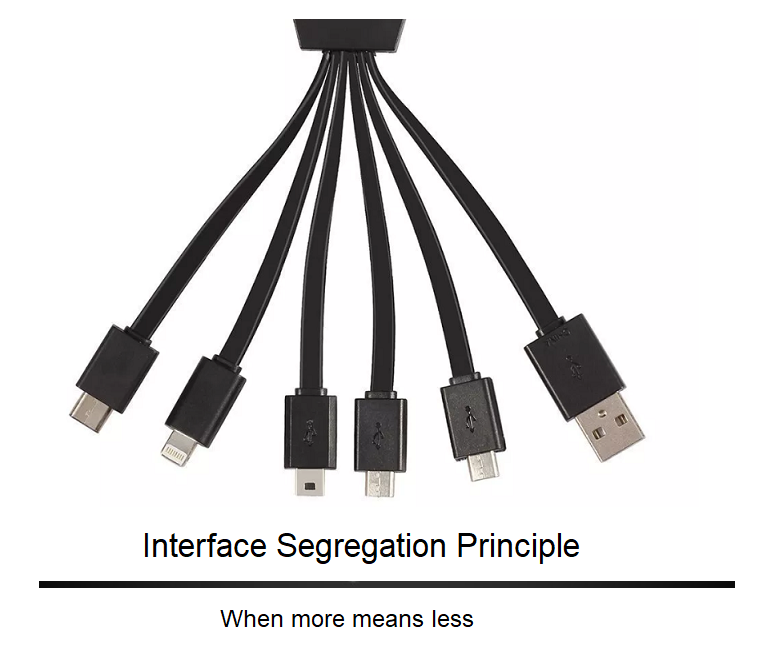
\includegraphics[width=0.5\linewidth]{PICs/ISP}
\caption{Interface segregation principle}\label{Abb1}
\end{figure}


\section{Interface}

An interface is a blueprint for an object and what it is capable of. In Object Oriented Programming, an Interface is a description of all functions that an object must have in order to be an "X". Again, as an example, anything that "ACTS LIKE" a light, should have a turnOn() method and a turnOff() method. The purpose of interfaces is to allow the computer to enforce these properties and to know that an object of TYPE T must have functions called X,Y,Z, etc. \cite{utah}


\section{ISP}

\begin{center} 
 ``Clients should not be forced to depend upon interfaces that they do not use.''\cite{ISP}\newline
\end{center} 

This principle was developed by Robert C. Martin while working at Xerox as a consultant. Martin was in charge of developing a new printing management system that could carry out tasks concurrently, which was new by the time.\cite{solidISP}

While developing this new printing system, Martin noticed that small changes in the design caused large-scale deployments. In some same cases caused deployments on modules out of the scope of the change. The problem was mainly caused by a large fat interface used throughout all the modules of the system.\cite{solidISP}

This principle is simple and clear, interfaces should not be forced to implement methods that they do not use. It has the main goal of limiting the scope of future changes. However, it is very difficult, in the first iterations, to identify the critical parts of your solution that will violate the principle. So, my advice is to wait for your code to evolve, so you can identify where you can apply it. Don't try to guess future requirements because there is a chance that you make your code more complicated.\cite{solidISP}


\section{Problem with will be solved with the ISP}
With ISP you can prevent overloaded interfaces that forces the client to implement a method that is not required. The client ends up implementing a usefulness method, in other words a method that has no meaning to the client. This decreases the readability of the code and also confuses the developer using the client code.
The client interface ends up violating SRP sometime since it might perform some action that is not related to it.\cite{csharpsolid}


\newpage

\chapter{Practical Example}

In the first example the Osterich class is forced to use the fly method. It is a clear violation of the Interface Segregation Principle. As you can see in the second example, the fly and walk methods were separated into an extra interface. With this implementation it is possible to use the fly and walk method at the Duck class and the walk method at the Ostrich class. Now no class is forced to implement an unused method. \newline

\begin{listing}[htbp]
\begin{minted}{java}
interface Bird {
  fly(): void;
  walk(): void;
}
class Duck extends Bird{
    fly(){
        // Duck can fly
    }   
    walk(){
        // Duck can walk
    }
}
class Ostrich extends Bird{
    fly(){
        // Ostrich cant fly... throw some error
    }   
    walk(){
        // Ostrich can walk
    }
}
\end{minted}
\caption{initial scenario}
\end{listing}

\newpage


\begin{listing}[htbp]
\begin{minted}{java}
interface BirdFly{
    fly(): void;
}
interface BirdWalk{
    walk(): void;
}
class Duck extends BirdFly, BirdWalk{
    fly(){
        // Duck can fly
    }   
    walk(){
        // Duck can walk
    }
}
class Ostrich extends BirdWalk{
    walk(){
        // Ostrich can walk
    }
}
\end{minted}
\caption{ISP Implementation}
\end{listing}



% Hier beginnen die Verzeichnisse.
\clearpage
\bibliographystyle{IEEEtran}
\bibliography{Literatur}
\clearpage

\listoffigures
\clearpage
\listoflistings
%Fix for fhtw_cover

\includegraphics[width=0\linewidth]{PICs/fhtw_cover}
\clearpage


\end{document}
